%%% File encoding is ISO-8859-1 (also known as Latin-1)
%%% You can use special characters just like �,� and �
%%% LaTeX template by Manuel Kuehner, 2015

%%% If you use this template then please give credit like this:
%%% ----------------------------
% LaTeX code inspired by the LaTeX Thesis Template by Manuel Kuehner 
% www.bedienhaptik.de/latex-template/
%%% ----------------------------

% ##############################################
% Start: Template Preamble
% ##############################################
%

% Documentclass definition
%%% File encoding is ISO-8859-1 (also known as Latin-1)
%%% You can use special characters just like �,� and �

% KOMA-Script class 'scrbook'
% Link to the documentation: 
% German: http://mirrors.ctan.org/macros/latex/contrib/koma-script/doc/scrguide.pdf
% English: http://mirrors.ctan.org/macros/latex/contrib/koma-script/doc/scrguien.pdf
% CTAN: http://www.ctan.org/pkg/koma-script
% Author of the KOMA-Script family is Markus Kohm
\documentclass%
[%
paper=a4
,fontsize=11pt % common are 10, 11 or 12
,headings=big
,parskip
,numbers=noendperiod % 2.3.1 vs 2.3.1. (no dot after the last chapter number)
,twoside=true
,toc=bibliography % Bibliography appears in Table of Contents (without a number)
,toc=listof % List of Figures and List of Tables appear in Table of Contents
,version=last % Use latest version of the KOMA-Script
]%
{scrbook}

% Loading additional packages from the KOMA-Script family
%%% File encoding is ISO-8859-1 (also known as Latin-1)
%%% You can use special characters just like �,� and �

% Special KOMA-Script package - I added it because I also use the float package in this template, see: 
% http://tex.stackexchange.com/questions/51867/koma-warning-about-toc
% CTAN: http://www.ctan.org/tex-archive/macros/latex/contrib/koma-script/doc
\usepackage{scrhack}

% Better support for marginnotes
% new command: \marginnote
% LaTeX standard command: \marginpar
% CTAN: http://www.ctan.org/pkg/marginnote
\usepackage{marginnote}

% Extended header and footer support
% CTAN: http://www.ctan.org/pkg/scrpage2
\usepackage[%
  	automark
  	,ilines
	,headsepline
	,footsepline
]{scrpage2}

% Page layout definition
%%% File encoding is ISO-8859-1 (also known as Latin-1)
%%% You can use special characters just like �,� and �

% User friendly interface to change layout parameters
% CTAN: http://www.ctan.org/pkg/geometry
\usepackage{geometry}
\geometry{% siehe geometry.pdf (Figure 1)
	bottom=30mm,
	showframe=false, % For debugging: try true and see the layout frames
	margin=30mm,
	marginparsep=3mm,
	marginparwidth=20mm
}

% Standard packages
%%% File encoding is ISO-8859-1 (also known as Latin-1)
%%% You can use special characters just like �,� and �

% Input encoding is 'latin1' (Latin 1 - also known as ISO-8859-1)
% CTAN: http://www.ctan.org/pkg/inputenc
% 
% A newer package is available - you may look into:
% \usepackage[x-iso-8859-1]{inputenc}
% CTAN: http://www.ctan.org/pkg/inputenx
\usepackage[latin1]{inputenc}

% Font Encoding is 'T1' -- important for special characters such as Umlaute � or � and special characters like � (enje)
% CTAN: http://www.ctan.org/pkg/fontenc
\usepackage[T1]{fontenc}

% Language support for 'english' (alternative 'ngerman' or 'french' for example)
% CTAN: http://www.ctan.org/pkg/babel
\usepackage[english]{babel} 

% Doing calculations with LaTeX units -- needed for the vertical line in the footer
% CTAN: http://www.ctan.org/pkg/calc
\usepackage{calc}

% Extended graphics support 
% There is also a package named 'graphics' - watch out!
% CTAN: http://www.ctan.org/pkg/graphicx
\usepackage{graphicx}

% Extendes support for floating objects (tables, figures), adds the [H] placing option (\begin{figure}[H]) which palces it "Here" (without any doubt).
% CTAN: http://www.ctan.org/pkg/float
\usepackage{float}

% Extended color support
% I use the command \definecolor for example. 
% Option 'Table': Load the colortbl package, in order to use the tools for coloring rows, columns, and cells within tables.
% CTAN: http://www.ctan.org/pkg/xcolor
\usepackage[table]{xcolor} 

% Nice tables
% CTAN: http://www.ctan.org/pkg/booktabs
\usepackage{booktabs}

% Better support for ragged left and right. Provides the commands \RaggedRight and \RaggedLeft. 
% Standard LaTeX commands are \raggedright and \raggedleft
% http://www.ctan.org/pkg/ragged2e
\usepackage{ragged2e}

% Create function plots directly in LaTeX
% CTAN: http://www.ctan.org/pkg/pgfplots
\usepackage{pgfplots}
\pgfplotsset{compat=1.11}
\usepackage{xcolor}
\usepackage{amsmath,amsthm,amsfonts}
\usepackage{fdsymbol}
\usepackage{graphicx}
\usepackage{scrextend}
\usepackage{multicol}
\usepackage{booktabs}
\usepackage{array}
\usepackage{tabularx}
\usepackage{changepage}
\usepackage{tcolorbox}
\tcbuselibrary{skins,breakable,theorems}

% ####-Important-####
%
% Definition of the two main colors
% -----------------------
% The corresponding xcolor package ist loaded in the file 
% 01_Preamble/StandardPackages.tex
%
% ####-Important-####
\definecolor[named]{myColorMainA}{RGB}{0,26,153}
\definecolor[named]{myColorMainB}{RGB}{174,49,54}

% Customization of 
% - Floating Objects (Caption) 
% - Table of Contents (TOC)
% - List of Figures
% - List of Tables
% - Headings (like chapter, section, etc.)
%%% File encoding is ISO-8859-1 (also known as Latin-1)
%%% You can use special characters just like �,� and �

% ##############################################
% Start: Table of Contents (TOC) Customization
% ##############################################
%

% Level for numbered captions
\setcounter{secnumdepth}{5}

% Level of chapters that appear in Table of Contents
\setcounter{tocdepth}{5} % bis wohin ins Inhaltsverzeichnis aufnehmen
% -2 no caption at all
% -1 part
% 0  chapter
% 1  section    
% 2  subsection 
% 3  subsubsection
% 4  paragraph
% 5  subparagraph

% KOMA-Script code to adjust TOC
% Applying the color 'myColorMainA' which is defined in the main file (MainFile.tex)
\makeatletter
\addtokomafont{chapterentrypagenumber}{\color{myColorMainA}}
\addtokomafont{chapterentry}{\color{myColorMainA}}
\makeatother

%
% #######################
% End: Table of Contents (TOC) Customization
% #######################

% ##############################################
% Start: Floating Object Customization
% ##############################################
%

% Extended support for catioons of figures and tables etc.
% CTAN: http://www.ctan.org/pkg/caption
\usepackage[%
	font={small},
	labelfont={bf,sf},
	format=hang, % try plain or hang
	margin=5pt,
]{caption}
%

% #######################
% End: Floating Object Customization
% #######################

% ##############################################
% Start: Headings Customization
% ##############################################
%

% KOMA-Script code to customize the headings
% Applying the color 'myColorMainA' which is defined in the main file (MainFile.tex)
\addtokomafont{chapter}{\color{myColorMainA}}
\addtokomafont{section}{\color{myColorMainA}}
\addtokomafont{subsection}{\color{myColorMainA}}
\addtokomafont{subsubsection}{\color{myColorMainA}}
\addtokomafont{paragraph}{\color{myColorMainA}}
\addtokomafont{subparagraph}{\color{myColorMainA}}

% #######################
% End: Headings Customization
% #######################


% Customization of the header, footer and teh margin note
%%% File encoding is ISO-8859-1 (also known as Latin-1)
%%% You can use special characters just like �,� and �

% Custom command fpr the margin notes: \myMarginnote{Your Text}
% Comment on the \lineskiplimit=-\maxdimen:
% See http://tex.stackexchange.com/questions/49072/
% Without it the line spacing of the normal text was changed (ugly).
\newcommand{\myMarginnote}[1]{%
	\marginnote{% needs marginnote package
		\ifthispageodd{\RaggedRight}{\RaggedLeft}% needs ragged2e package
		\color{myColorMainB}%
		\lineskiplimit=-\maxdimen% 
		\normalfont\sffamily\scriptsize%
		#1}%
}


\DeclareRobustCommand{\examplebox}[2][gray!10]{%
\begin{tcolorbox}[   %% Adjust the following parameters at will.
        breakable,
        left=0pt,
        right=0pt,
        top=0pt,
        bottom=0pt,
        colback=#1,
        colframe=#1,
        width=\dimexpr\textwidth\relax-10mm, 
        enlarge left by=10mm,
        boxsep=3pt,
        arc=0pt,outer arc=0pt,
        ]
        #2
\end{tcolorbox}
}
% ##############################################
% Start: Header and Footer Customization
% ##############################################
%

% KOMA-Script code for header and footer font
\setkomafont{pageheadfoot}{%
	\normalfont\sffamily\bfseries
	}
\setkomafont{pagefoot}{%
	\normalfont\sffamily
	}
\setkomafont{pagenumber}{%
	\normalfont\rmfamily
	}

% Define width of header
\setheadwidth[0pt]{textwithmarginpar}

% Define with of header line
\setheadsepline{0.4pt}

% Define width of footer
\setfootwidth[0pt]{text}
% Define with of footer line (here: no line)
\setfootsepline[text]{0pt}

% Some calculations
% calc package is needed which is loaded here: 01_Preamble/CommonPackages.tex
% If you want to understand the calculations visit:
% http://en.wikibooks.org/wiki/LaTeX/Page_Layout
\newlength{\myLenghthFootAbstand}
\setlength{\myLenghthFootAbstand}{\paperheight-1in-\topmargin- \headheight-\headsep-\textheight-\footskip}
\newlength{\myLenghthTemp}
\setlength{\myLenghthTemp}{\myLenghthFootAbstand+\baselineskip}

% Define content of header and footer
% Using some scrpage2 commands here. The scrpage2 package is loaded here: 01_Preamble/KOMA-Script-Packages.tex
% Some LaTeX magic...
% Clear all defaults
\clearscrheadfoot
% Header
\ohead{%
	\textcolor{myColorMainA}{\headmark}
	}
% Left (even page numbers) footer
\lefoot%
[% scrplain style (begin)
	\setlength{\unitlength}{\myLenghthFootAbstand}%
	\begin{picture}(0,0)%
		\put(0,-1)%
		{%
			\makebox(0,0)[lb]%
			{%
				\rule{0.4pt}{\myLenghthTemp}%
			}%
		}%
	\end{picture}\llap{\pagemark~}%
]% scrplain style (end)
%
{% scrheadings style (begin)
	\setlength{\unitlength}{\myLenghthFootAbstand}%
	\begin{picture}(0,0)%
		\put(0,-1)%
		{%
			\makebox(0,0)[lb]%
			{%
				\rule{0.4pt}{\myLenghthTemp}%
			}%
		}%
	\end{picture}\llap{\pagemark~}%
}% scrheadings style (end)

% Right (odd page numbers) footer
\rofoot%
[% scrplain style (begin)
	\rlap{~\pagemark}%%
	\setlength{\unitlength}{\myLenghthFootAbstand}%
	\begin{picture}(0,0)%
		\put(0,-1)%
		{%
			\makebox(0,0)[lb]%
			{%
				\rule{0.4pt}{\myLenghthTemp}%
			}%
		}%
	\end{picture}%
]% scrplain style (end)
%
{% scrplain style (begin)
	\rlap{~\pagemark}%%
	\setlength{\unitlength}{\myLenghthFootAbstand}%
	\begin{picture}(0,0)%
		\put(0,-1)%
		{%
			\makebox(0,0)[lb]%
			{%
				\rule{0.4pt}{\myLenghthTemp}%
			}%
		}%
	\end{picture}%
}% scrplain style (end)

%
% #######################
% End: Header and Footer Customization
% #######################

% Optimize paragraphs (avoid overfull... warnings)
%%% File encoding is ISO-8859-1 (also known as Latin-1)
%%% You can use special characters just like �,� and �

% This is an suggestion from Axel Reichert (LaTeX package author)
% See CTAN: http://www.ctan.org/author/reichert
% See CTAN: http://www.ctan.org/pkg/l2tabu-english (Cgapter: 1.8 Should I use \sloppy?)

\tolerance 1414
\hbadness 1414
\emergencystretch 1.5em
\hfuzz 0.3pt
\widowpenalty=10000
\vfuzz \hfuzz
\raggedbottom

% PDF related packages
%%% File encoding is ISO-8859-1 (also known as Latin-1)
%%% You can use special characters just like �,� and �

% Package for PDF features such as bookmarks and hyperlinks. 
% Important: Should be loaded at the end.
% CTAN: http://www.ctan.org/pkg/hyperref
\usepackage[%
bookmarks, % Create bookmarks
bookmarksopen=true, % Unfold bookmatk tree in PDF viewer when document is opened
bookmarksopenlevel=1, % Level of unfolding
bookmarksnumbered=true, % Number bookmarks
hidelinks, % do not highlight hyperlinks -- looks ugly
% Ansicht beim �ffnen
pdfpagelabels=true, % See manual...
plainpages=false, % See manual...
hyperfootnotes=true, % Hyperlinks for footnotes
hyperindex=true, % Indexeintr�age verweisen auf Text
]{hyperref}


% Custom macros
\newcommand{\highlight}[1]{\textbf{\textsf{\textcolor{myColorMainA}{#1}}}}
\newcommand{\symbdefbox}[2]{\highlight{#1 #2}\mathmarginbox{#2}}
\newcommand{\mathmarginbox}[1]{\myMarginnote{\scalebox{1.5}{\ifthispageodd{$\blacktriangleleft$}{\null} #1 \ifthispageodd{\null}{$\blacktriangleright$}}}}
\newcommand{\example}[1]{\small\examplebox{\textit{Example:} #1}}
% #######################
% Ende: Template Preamble
% #######################

% ##############################################
% Start: Document
% ##############################################
%
% ------------------------------------------------------------------
\begin{document}

% Title page
%%% File encoding is ISO-8859-1 (also known as Latin-1)
%%% You can use special characters just like �,� and �

% Title page using \maketitle (a more flexible alternative is the titlepage environment)
\title{Algorithmic Foundations of Datascience}
\subtitle{A summary of the Lecture}
\author{Felix Friedberger}
\date{April 2019 - September 2019}
\maketitle
% Empty page after title page
\cleardoublepage

% Activate header and footer defined in the file:
% 01_Preamble/HeaderFooterMarginnote.tex
\pagestyle{scrheadings}

% Activate roman numbering (e. g. xii)	
\pagenumbering{roman}

% Start with page 1 (I)
\setcounter{page}{1}


% Abstract
%%% File encoding is ISO-8859-1 (also known as Latin-1)
%%% You can use special characters just like �,� and �

% Chapter without numbering but with appearance in the Table of Contents
% \addchap is a command from KOMA-Script
\addchap{Abstract}

This summary is based on the lecture 'Algorithmic Foundations of Datascience' held by Prof. Martin Grohe in the summer term of 2019 at RWTH Aachen University.\newline

Since this summary is made by student(s), there are definitely mistakes in the script. Should you find one feel free to contact me.

% Table of Contents and Lost of Figures/Tables
%%% File encoding is ISO-8859-1 (also known as Latin-1)
%%% You can use special characters just like �,� and �

% Table of Contents (TOC)
% Special code so that it appears as a bookmark in the PDF viewer
\phantomsection
\pdfbookmark[0]{Table of Contents}{toc} % <-- Please edit the name if you want a different text as a bookbarl for the Table of Contents
\tableofcontents
% List of Figures
%\listoffigures
% List of Tables
%\listoftables 

% Activate arabic numbering (e. g. 12)	
\pagenumbering{arabic}

% Start with page 1
\setcounter{page}{1}

% Introduction
%%% File encoding is ISO-8859-1 (also known as Latin-1)
%%% You can use special characters just like �,� and �

\chapter{Machine Learning Basics}

\section{Definitions}
All the following definitions are specific to 'Machine Learning' and might change throughout the summary.


\highlight{Data} is viewed as a collection of data items (or dataset). A \highlight{data item} is represented by a so-called feature vector. The \highlight{feature vector} basically a list of features and attributes in form of a vector 
\subsection{Domains}
The \symbdefbox{Domain}{$\mathbb{D}$} is a set containing the range of all possible values for a single feature. The \symbdefbox{Instance Space}{$\mathbb{X}$} is the Cartesian product of the domains of all features in the feature vector. The number of features is the dimension of the instance space (or the number of entries in the feature vector). 
\example{The domain space can be something like $\{true,false\}$ or $\mathbb{N}$, aso. The instance space of the domain spaces is then (informally) $\mathbb{D}_1\times \mathbb{D}_2 \times \ldots \times \mathbb{D}_l$}
Assuming $n$ is the number of data items, and $l$ the number of features the whole dataset can be viewed as an $(n \times l )$-matrix over the instance space.

\section{Forms of Learning}
\highlight{Unsupervised learning} tries to detect patterns in data with, hence the name, no feedback, supplied the Learning algorithm. This technique is mostly used for clustering.

\highlight{Reinforcement Learning} tries to find actions that maximise reward. The feedback to the learning algorithm is provided in form of a reward (or punishment)

In \highlight{Supervised learning} one tries to approximate a function by training on input-output pairs. \highlight{Classification} has a finite-valued function and tries to predict values for future inputs. \highlight{Regression} has a numerical function and tries to predict the expected values for future inputs. Supervised learning can be differentiated into two different set-ups. First, \highlight{Batch Learning}, in which all examples are supplied at once and the learner has to come up with a hypothesis. Where as in \highlight{Online Learning}, examples are given 'on-the-fly' once at a time and the initial hypothesis gets improved over time.

\highlight{Semi-supervised Learning} is similar to supervised learning, but takes only a few and possibly faulty examples and tries to make the best of the possibly small and faulty dataset.

%TODO: Add Active/Passive Learning

\section{Hypothesis Space}
In Supervised learning, the unknown target function $h$ is choosen from the \symbdefbox{hypothesis space}{$\mathcal{H}$}, hence $h \in \mathcal{H}$. The Hypothesis space contains all linear functions, all polynomials or all polynomials of a pre-scribed degree, and all functions that can be described by a decision tree.

A learning problem is \highlight{Realisable} if the target function $h$ is in the Hypothesis Space.
\example{Assuming a target function $h(x):= a \cdot sin(x) + bx + c$. Then, if $\mathcal{H}$ only contains polynomials, the learning problem is \textbf{not realizable}. But, assuming $\mathcal{H}$ contains linear functions or polynomials in $x$ and $sin(x)$, the learning problem \textbf{is realisable}.}

\section{Validation}
The goal of the learning algorithm is to produce a hypothesis that generalizes well, that is, approximates the target function well ion the all data points (and not only those in the training set). To evaluate how well a hypothesis generalizes we can evaluate it against some test set. A \highlight{test set} is generates by splitting the examples into a test set and training set.

The Empirical Observation that simpler hypothesis tend to generalise better is picked up by \highlight{Occam's Razor} which states, that the simplest hypothesis which is consistent with the data should be choosen.

\highlight{Overfitting} is the phenomenon, which occurs when the leaner tries to match the training examples as exactly as possible which leads to complex hypotheses that generalize badly. Thus, to avoid overfitting, it is often better to choose a simple hypothesis even if it doesn't match the data exactly.

\section{Nearest Neighbour Learning}
The underlying idea of this simple learning algorithm is to predict the value of a function at point $x$ by looking at known values of points close to the given one and assume the value of $x$ is similar. 
\subsection{Metric}
A \symbdefbox{metric}{$d$} on $\mathbb{X}$ is a function $d: \mathbb{X}^2 \longrightarrow  \mathbb{R}$ such that for all $x,y,z \in \mathbb{X}$

\newlength\q
\setlength\q{\dimexpr .33\textwidth -2\tabcolsep}
\begin{tabular}{p{\q}|p{\q}|p{\q}}
	\highlight{Nonnegativity} & \highlight{Symmetry} & \highlight{Triangle Inequality}\\
	$\begin{aligned} &d(x,y) \geq 0 \\	\texttt{and }  &d(x,y) = 0 \Longleftrightarrow x=y;\end{aligned}$ & 	$d(x,y) = d(y,x)$ &  $d(x,z) \leq d(x,y) + d(y,z)$\\
\end{tabular}


\subsection{Metric Spaces}
Suppose $\mathbb{X}$ is the instance space, and $d$ be some metric on $\mathbb{X}$. Then we have a \symbdefbox{Metric Space}{$(\mathbb{X},d)$}.

\subsubsection{Common distance metrics}
The distance between points $x$ and $y$ is denoted as $d(x,y)$\mathmarginbox{$d(x,y)$}.

\highlight{Euclidean distance} with $\mathbb{X} = \mathbb{R}^l$:
\begin{equation}
d(x,y) = \sqrt{\sum^{l}_{i=1} (x_i - y_i)^2}
\end{equation}

\highlight{Manhattan distance} with $\mathbb{X} = \mathbb{R}^l$:
\begin{equation}
d(x,y) = \sum^{l}_{i=1}|x_i-y_i|
\end{equation}

\highlight{Hamming distance} with $\mathbb{X} = \mathbb{D}_1 \times \mathbb{D}_2 \times \ldots \times \mathbb{D}_l$
\begin{equation}
d(x,y) = |\{\,i\,|\, x_i \neq y_i\}|
\end{equation}

% Main Part
%%% File encoding is ISO-8859-1 (also known as Latin-1)
%%% You can use special characters just like �,� and �

\chapter{Main Part}

%\Blindtext[1][1]

\begin{figure}[H]
\centering
	\includegraphics[width=0.9\textwidth]%
	{src/03_GraphicFiles/CowLickingNose.jpg}%
\caption[A cow]{A cow licking its nose. Usage with permission of the photographer \textsc{Nicole Barth}, taken from \url{www.flickr.com/photos/46311827@N07/14885545396}.}
\label{fig:CowLickingNose}
\end{figure}

In \figurename~\ref{fig:CowLickingNose}\myMarginnote{Reference to a figure} you see a cow that is licking its nose. The picture was taken by Nicole Barth on 11.08.2014 using a Canon EOS 500D. The original file has a resolution of $4247 \times 2831$ pixels.

\begin{figure}[H]
\centering
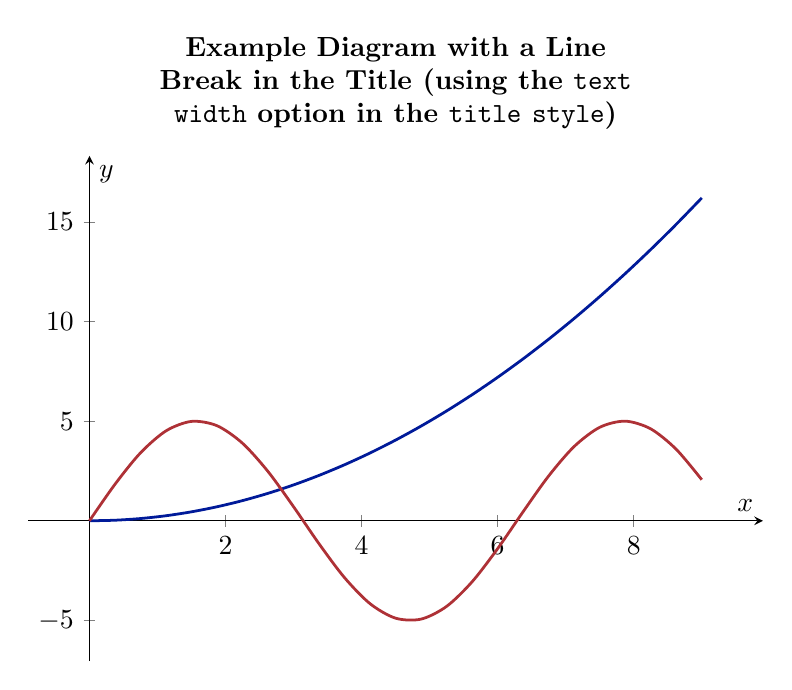
\begin{tikzpicture}
\begin{axis}[
axis lines = middle,
enlargelimits = true,
xlabel = {$x$},
ylabel = {$y$},
trig format plots = rad,
width = 0.9\textwidth,
height= 80mm,
title style={font=\bfseries,align=center,text width=0.7\textwidth},
title = {Example Diagram with a Line Break in the Title (using the \texttt{text width} option in the \texttt{title style})},
]
\addplot[myColorMainA,domain=0:9, line width=1pt, smooth]
{0.2*x^2};
\addplot[myColorMainB,domain=0:9, line width=1pt, smooth]
{5*sin(x)};
\end{axis}
\end{tikzpicture}
\caption[Scientific diagram]{A scientific diagram using the \texttt{pgfplots} package by \textsc{Christian Feuersaenger} using the same colors which are also used for the layout.}
\label{fig:ScientificDiagram}
\end{figure}

%\Blindtext[2][2]

\begin{table}[H]
\centering
\begin{tabular}{@{}llr@{}} \toprule
\multicolumn{2}{c}{Item} \\ \cmidrule(r){1-2}
Animal & Description & Price (\$)\\ \midrule
Gnat & per gram & 13.65 \\
& each & 0.01 \\
Gnu & stuffed & 92.50 \\
Emu & stuffed & 33.33 \\
Armadillo & frozen & 8.99 \\ \bottomrule
\end{tabular}
\caption[Small table]{A small table created with the \texttt{booktabs} package (example taken from the package documentation).}
\end{table}


%\Blindtext[2][1]

\section{Example Section}

%\Blindtext[3][2]

%\blinditemize

\section{Another Example Section}

%\Blindtext[3][1]

%\blindenumerate

\subsection{Example Sub-Section}

%\blindmathpaper

\begin{figure}[H]
\centering
	\includegraphics[]%
	{src/03_GraphicFiles/CowLickingNoseSquare.jpg}%
\caption[A cow (square)]{A cow licking its nose -- picture in square format in a native (low) resolution $150 \times 150$ pixels @ 72~dpi ($\approx 2.1$ inch). No scaling in \LaTeX{} using options in \texttt{\textbackslash includegraphics} is applied. Zoom in and see how ugly this is. See \figurename~\ref{fig:CowLickingNose} for reference.}.
\label{fig:CowLickingNoseSquare}
\end{figure}

\subsection{Another Example Sub-Section}

%\Blindtext[2][1]

\subsubsection{Another Sub-Sub-Section}

%\blindmathpaper

\paragraph{Example Paragraph}

%\Blindtext[2][1]

\subparagraph{Example Sub-Paragraph}

%\Blindtext[2][1]

\section{Yet Another Example Section}

%\Blindtext[2][1]

% Final Thoughts
%%% File encoding is ISO-8859-1 (also known as Latin-1)
%%% You can use special characters just like �,� and �

\chapter{Final Thoughts}

%\Blindtext[2][1]


\end{document}
% ------------------------------------------------------------------
%
% #######################
% End: Document
% #######################
